\chapter{Approaches to Time Series compression}
\section{Storing aggregates}
Storing aggregates is probably the most common approach to deal with large time series.
The idea is to reduce the temporal resolution of data by storing aggregates of values within
some predefined time buckets. Once values have been aggregated to a lower temporal resolution,
they can be deleted, provided that the initial temporal resolution is not needed anymore.
As a practical example, let us consider an application in which we record the time delays
accumulated by trains. The following series represent the daily delay of a specific train on
a certain day in minutes.
\begin{table}[!htbp]
\centering
\begin{tabular}{l|l|l|l|l|l|l}
\textbf{Day 1} & \textbf{Day 2} & \textbf{Day 3} & \textbf{Day 4} & \textbf{Day 5} & \textbf{Day 6} & \textbf{Day 7} \\
\hline
20 & 20 & 10 & 50 & 40 & 40 & 30 \\                
\end{tabular}
\caption{Daily delay of a specific train of a certain day in minutes.}
\label{tab:daily_delay}
\end{table}

After each week passes, we want to aggregate the previous week’s daily data. With reference
to our example above, we can delete the daily values and replace them by their sum
(210 minutes). By also storing the count, we can compute the average daily during that week
(210 / 7 = 30 minutes).
This technique, often called downsampling, is so simple and effective that most time series
databases offer it out of the box. For example, OpenTSDB, an open-source time series database,
offers the possibility to query downsampled data \cite{A2019Downsample}. This is useful when
one wants to plot data keeping the density at a level that can be easily understandable by
users. Admittedly, this feature does not hold any savings in terms of storage, as it is
performed only at query time, but it is still interesting for network bound applications.
Since version 2.4 OpenTSDB offers the possibility to store the result of the downsampler
\cite{A2019Rollup}. In this way, when querying for a long time span, there is no need to wait for the
downsampled data to be computed.
InfluxDB, another popular open-source database, offers the possibility to downsample old
data using continuous queries and retention policy \cite{A2016Downsampling}. Continuous queries
are queries that are run automatically and periodically within a database. Retention policy
defines for how long InfluxDB keeps the data. By using these concepts together, one can use
a continuous query to aggregate old data into a lower temporal resolution and delete the
original data automatically by setting an appropriate retention policy.

\section{Lossless compression}
Lossless compression is a method of data compression that allows to reconstruct the original
data from the compressed data \cite{WikipediaContributors2019Data}. When applied to time series, it is used when we are
interested in retaining the original data but we want to reduce storage space. In this
section, we will present two different algorithms that have been devised to solve different
problems. The first algorithm was created at Facebook to face the huge amount of data
gathered by monitoring their systems. This algorithm has allowed them to store all data
in memory, thus improving considerably reading and writing performance.
The second algorithm we present, called Sprintz, was created to limit the energy consumption
of IoT devices. By sending compressed data, the network interface use is reduced, thus
obtaining considerable power savings.

\subsection{Gorilla}
Gorilla is an in-memory time series database used by facebook for monitoring the health of
their systems. It was initially presented in a 2015 paper, and it is now available as
open-source software under the name of Beringei \cite{beringei}. Gorilla schema is a simple tuple
composed of three values: the key of the time series stored as a string, the timestamp of the
measurement stored as an integer, and the value stored as a double. 
The compression is applied both to the timestamp and the actual double values. For the
timestamp the delta-of-delta technique is used (which we discussed in chapter 2), while for
the double values a special kind of XOR compression is applied.

\subsubsection{Timestamp compression}
Timestamp compression is achieved by storing the delta of deltas (see previous chapter)
together with a variable-length code.
The algorithm can be described as follows:
\begin{enumerate}
    \item in the block header, we store the initial timestamp $t-1$ which is aligned to a
    two-hour window. The first timestamp $t_0$ is stored as a 14-bit delta from $t-1$.
    \item For the subsequent timestamp $t_n$:
        \begin{enumerate}
            \item calculate the delta of delta $D = (t_n - t_{n-1}) - (t_{n-1} - t_{n-2})$
            \item if delta is 0, store ‘0’
            \item if delta is between [-64, 64], store ‘10’ following the 7-bit value of the
            delta
            \item if delta is between [-256, 256], store ‘110’ following with the 9-bit
            value of the delta
            \item if delta is between [-2048, 2048], store ‘1110’ following the 12-bit value
            of the delta
            \item otherwise, store ‘1111’ followed by the 32-bit value
        \end{enumerate}
\end{enumerate}
This type of compression applied to Facebook experimental data was able to achieve a 96\%
compression ratio. Figure~\ref{gorilla_timestamp} shows the result of the timestamp
compression achieved by Gorilla with Facebook’s data. It is interesting to note that
96\% of the time timestamps were compressed in one bit.

\begin{figure}[]
\begin{center}
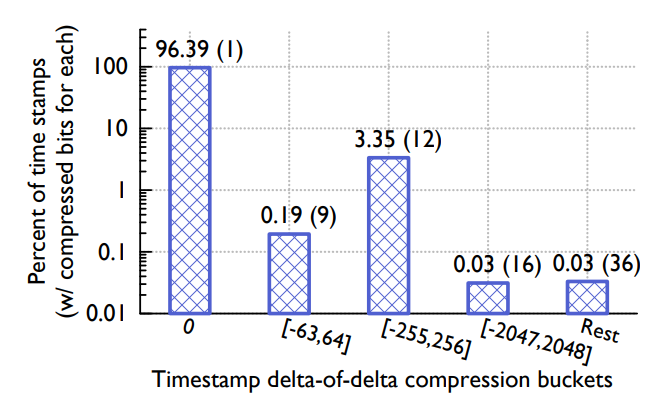
\includegraphics[width=200pt]{gorillaTimestamp}
\caption[gorilla_timestamp]{ Distribution of timestamp compression across different ranged buckets.
Taken from a sample of 440,000 real timestamps in Gorilla \cite{Pelkonen2015Gorilla}}
\label{gorilla_timestamp}
\end{center}
\end{figure}

\subsubsection{Compressing values}
Gorilla restricts the value element in its tuple to a double floating-point type. To compress
the values, XOR compression is used together with a variable-length code.
Since values that are close together do not differ by a large amount, the sign, exponent and
few bits of the mantissa are usually the same. Gorilla exploits this by computing the XOR of
the current and previous values. We XOR’d values are then encoded using the following encoding
scheme:
\begin{enumerate}
    \item the first value is stored with no compression
    \item if the XOR with the previous value is 0, then store ‘0’
    \item when XOR is non-zero, calculate the number of leading and trailing zeros in the XOR,
    store bit ‘1’ followed by either a) or b):
        \begin{enumerate}
            \item (control bit ‘0’) If the block of meaningful bits falls within the block of
            previous meaningful bits, i.e., there are at least as many leading zeros and as many
            trailing zeros as with the previous value, use that information for the block position
            and just store the meaningful XORed value
            \item (control bit ‘1’) Store the length of the number of leading zeros in the next
            5 bits, then store the length of the meaningful XORed value in the next 6 bits.
            Finally, store the meaningful bits of the XORed value
        \end{enumerate}
\end{enumerate}
We show an example of this coding in Table~\ref{tab:gorilla}.

\begin{table}[]
\centering
\begin{tabular}{p{1.5cm}|p{3.75cm}|p{4cm}|p{3.5cm}}
\textbf{Decimal} & \textbf{Double \newline representation} & \textbf{XOR with \newline previous} & \textbf{Encoded value} \\ 
\hline
20.5  & 0x4034800000000000 & -                  & 0b010000000011010 \newline 01000000000000000 \newline 00000000000000000 \newline 000000000000000 \\
18    & 0x4032000000000000 & 0x0006800000000000 & 0b110001100000010 \newline 1000100 \\ 
21.5  & 0x4035800000000000 & 0x0007800000000000 & 0b101001110                    \\              
21    & 0x4035000000000000 & 0x0000800000000000 & 0b101000                    \\           
21.25 & 0x4035400000000000 & 0x0000C00000000000 & 0b101100                    \\            
21.25 & 0x4035400000000000 & 0x0000000000000000 & 0b0                    \\            
\end{tabular}
\caption{An example of Gorilla's value compression.}
\label{tab:gorilla}
\end{table}

Using their data set, the authors of Gorilla noted that 51\% of the time subsequent values do
not change at all so they can be stored with one bit (case 2), while 30\% of the time they
have as much leading and trailing zeroes as the previous XOR’d value (case 3a), while the
remaining 19\% are stored with the ‘11’ prefix (case 3b), with an average size of 36.9 bits
due to the 13 bits extra overhead.

\subsection{Sprintz}